%%%%%%%%%%%%%%%%%%%%%%%%%%%%%%%%%%%%%%%%%%%%%%%%%%%%%%%%%%
%%%%%%%%%%%%%%%%%%%%%%%%%%%%%%%%%%%%%%%%%%%%%%%%%%%%%%%%%%
\subsection{Motivations}
%%%%%%%%%%%%%%%%%%%%%%%%%%%%%%%%%%%%%%%%%%%%%%%%%%%%%%%%%%
%%%%%%%%%%%%%%%%%%%%%%%%%%%%%%%%%%%%%%%%%%%%%%%%%%%%%%%%%%

%%%%%%%%%%%%%%%%%%%%%%%%%%%%%%%%%%%%%%%%%%%%%%%%%%%%%%%%%%
\frame {\frametitle{Collocate data and computation!}
%%%%%%%%%%%%%%%%%%%%%%%%%%%%%%%%%%%%%%%%%%%%%%%%%%%%%%%%%%
  \begin{itemize}
  \item \textbf{As dataset sizes increase, more computing capacity is
      required for processing}

    \vspace{20pt}

  \item \textbf{As compute capacity grows, the link between the
      compute nodes and the storage nodes becomes a bottleneck}
    \begin{itemize}
    \item One could eventually think of special-purpose interconnects
      for high-performance networking
    \item This is often a costly solution as cost does not increase
      linearly with performance
    \end{itemize}

    \vspace{20pt}

  \item \textbf{{\color{red}Key idea}: abandon the separation between
      compute and storage nodes}
    \begin{itemize}
    \item This is exactly what happens in current implementations of
      the MapReduce framework
    \item A distributed filesystem is not mandatory, but highly desirable
    \end{itemize}
  \end{itemize}
}

%%%%%%%%%%%%%%%%%%%%%%%%%%%%%%%%%%%%%%%%%%%%%%%%%%%%%%%%%%
\frame {\frametitle{The Hadoop Distributed Filesystem}
%%%%%%%%%%%%%%%%%%%%%%%%%%%%%%%%%%%%%%%%%%%%%%%%%%%%%%%%%%
  \begin{itemize}
  \item \textbf{Large dataset(s) outgrowing the storage capacity of a single
      physical machine}
    \begin{itemize}
    \item Need to partition it across a number of separate machines
    \item Network-based system, with all its complications
    \item Tolerate failures of machines
    \end{itemize}

    \vspace{20pt}

  \item \textbf{Distributed filesystems are not new!}
    \begin{itemize}
    \item HDFS builds upon previous results, tailored to the specific
      requirements of MapReduce
    \item {\color{red}Write once, read many workloads}
    \item Does not handle concurrency, but allow replication
    \item Optimized for throughput, not latency
    \end{itemize}

    \vspace{20pt}

  \item \textbf{Hadoop Distributed Filesystem\cite{shvachko10, hadoop_book}}
    \begin{itemize}
    \item Very large files
    \item Streaming data access
    \item Commodity hardware
    \end{itemize}
  \end{itemize}
}

%%%%%%%%%%%%%%%%%%%%%%%%%%%%%%%%%%%%%%%%%%%%%%%%%%%%%%%%%%
%%%%%%%%%%%%%%%%%%%%%%%%%%%%%%%%%%%%%%%%%%%%%%%%%%%%%%%%%%
\subsection{Blocks}
%%%%%%%%%%%%%%%%%%%%%%%%%%%%%%%%%%%%%%%%%%%%%%%%%%%%%%%%%%
%%%%%%%%%%%%%%%%%%%%%%%%%%%%%%%%%%%%%%%%%%%%%%%%%%%%%%%%%%

%%%%%%%%%%%%%%%%%%%%%%%%%%%%%%%%%%%%%%%%%%%%%%%%%%%%%%%%%%
\frame {\frametitle{HDFS Blocks}
%%%%%%%%%%%%%%%%%%%%%%%%%%%%%%%%%%%%%%%%%%%%%%%%%%%%%%%%%%
  \begin{itemize}
  \item \textbf{(Big) files are broken into block-sized chunks}
    \begin{itemize}
    \item Blocks are big! [64, 128] MB
    \item Avoids problems related to metadata management
    \item \texttt{NOTE}: A file that is smaller than a single block {\color{red}does not} occupy a full block's worth of underlying storage
    \end{itemize}

\vspace{20pt}

  \item \textbf{Blocks are stored on independent machines}
    \begin{itemize}
    \item Replicate across the local disks of nodes in the cluster
    \item Reliability and parallel access
    \item Replication is handled by storage nodes themselves (similar
      to \textbf{chain replication})
    \end{itemize}

\vspace{20pt}

  \item \textbf{Why is a block so large?}
    \begin{itemize}
    \item Make transfer times larger than seek latency
    \item E.g.: Assume seek time is 10ms and the transfer rate is 100
      MB/s, if you want seek time to be 1\% of transfer time, then the
      block size should be 100MB
    \end{itemize}
  \end{itemize}

}

%%%%%%%%%%%%%%%%%%%%%%%%%%%%%%%%%%%%%%%%%%%%%%%%%%%%%%%%%%
%%%%%%%%%%%%%%%%%%%%%%%%%%%%%%%%%%%%%%%%%%%%%%%%%%%%%%%%%%
\subsection{Architecture}
%%%%%%%%%%%%%%%%%%%%%%%%%%%%%%%%%%%%%%%%%%%%%%%%%%%%%%%%%%
%%%%%%%%%%%%%%%%%%%%%%%%%%%%%%%%%%%%%%%%%%%%%%%%%%%%%%%%%%

%%%%%%%%%%%%%%%%%%%%%%%%%%%%%%%%%%%%%%%%%%%%%%%%%%%%%%%%%%
\frame {\frametitle{NameNodes and DataNodes}
%%%%%%%%%%%%%%%%%%%%%%%%%%%%%%%%%%%%%%%%%%%%%%%%%%%%%%%%%%
  \begin{itemize}
  \item \textbf{\texttt{NameNode}}
    \begin{itemize}
    \item Keeps metadata {\color{red}in RAM}
    \item Each block information occupies roughly 150 bytes of memory
    \item Without \texttt{NameNode}, the filesystem cannot be used
      \begin{itemize}
      \item Persistence of metadata: synchronous and atomic writes to
        NFS
      \end{itemize}
    \item Maintains overall {\color{red}health} of the file system
    \end{itemize}

    \vspace{20pt}

  \item \textbf{\texttt{Secondary NameNode}}
    \begin{itemize}
    \item Merges the namespace with the edit log
    \item A useful trick to recover from a failure of the
      \texttt{NameNode} is to use the NFS copy of metadata and 
      switch the secondary to primary
    \end{itemize}

    \vspace{20pt}

  \item \textbf{\texttt{DataNode}}
    \begin{itemize}
    \item They store data and talk to clients
    \item They report periodically to the \texttt{NameNode} the list
      of blocks they hold
    \end{itemize}

  \end{itemize}
}

%%%%%%%%%%%%%%%%%%%%%%%%%%%%%%%%%%%%%%%%%%%%%%%%%%%%%%%%%%
\frame {\frametitle{Architecture Illustration}
%%%%%%%%%%%%%%%%%%%%%%%%%%%%%%%%%%%%%%%%%%%%%%%%%%%%%%%%%%
  \begin{figure}[h]
    \centering
    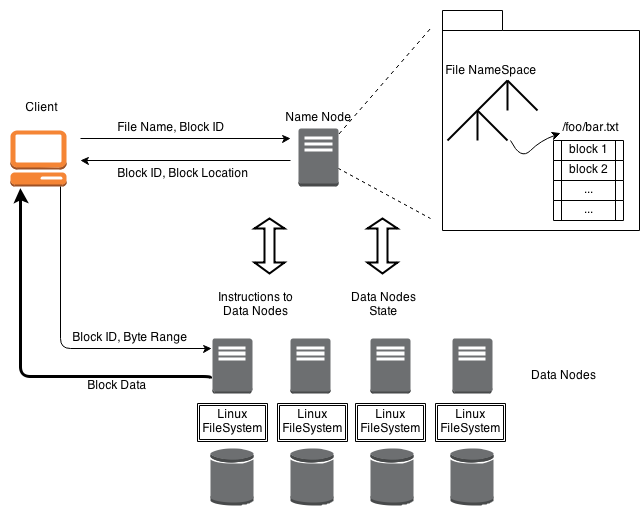
\includegraphics[scale=0.36]{./Figures/hdfs}
    \caption{Architecture sketch of HDFS operations.}
    \label{fig:hdfs}
  \end{figure}
}


%%%%%%%%%%%%%%%%%%%%%%%%%%%%%%%%%%%%%%%%%%%%%%%%%%%%%%%%%%
\frame {\frametitle{Anatomy of a File Read}
%%%%%%%%%%%%%%%%%%%%%%%%%%%%%%%%%%%%%%%%%%%%%%%%%%%%%%%%%%
  \begin{itemize}
  \item \textbf{\texttt{NameNode} is only used to get block location}
    \begin{itemize}
    \item Unresponsive \texttt{DataNode} are discarded by clients
    \item Batch reading of blocks is allowed
    \end{itemize}

    \vspace{20pt}

  \item \textbf{``External'' clients}
    \begin{itemize}
    \item For each block, the \texttt{NameNode} returns {\color{red}a
        set} of \texttt{DataNodes} holding a copy thereof
    \item \texttt{DataNodes} are sorted according to their proximity
      to the client
    \end{itemize}

    \vspace{20pt}

  \item \textbf{``MapReduce'' clients}
    \begin{itemize}
    \item \texttt{TaskTracker} and \texttt{DataNodes} are
      {\color{red}collocated}
    \item For each block, the \texttt{NameNode}
      usually\footnote{Exceptions exist due to stragglers.} returns
      the local \texttt{DataNode}
    \end{itemize}

  \end{itemize}
}

%%%%%%%%%%%%%%%%%%%%%%%%%%%%%%%%%%%%%%%%%%%%%%%%%%%%%%%%%%
\frame {\frametitle{Anatomy of a File Write}
%%%%%%%%%%%%%%%%%%%%%%%%%%%%%%%%%%%%%%%%%%%%%%%%%%%%%%%%%%
  \begin{itemize}
  \item \textbf{Details on replication}
    \begin{itemize}
    \item Clients ask \texttt{NameNode} for a list of suitable
      \texttt{DataNodes}
    \item This list forms a \texttt{pipeline}: first \texttt{DataNode}
      stores a copy of a block, then forwards it to the second, and so
      on
    \end{itemize}

    \vspace{40pt}

  \item \textbf{Replica Placement}
    \begin{itemize}
    \item {\color{red}Tradeoff} between reliability and bandwidth
    \item Default placement:
      \begin{itemize}
      \item First copy on the ``same'' node of the client, second
        replica is {\color{red}off-rack}, third replica is on the same
        rack as the second but on a different node
      \item Since Hadoop 0.21, replica placement can be customized
      \end{itemize}
    \end{itemize}

  \end{itemize}

}

%%%%%%%%%%%%%%%%%%%%%%%%%%%%%%%%%%%%%%%%%%%%%%%%%%%%%%%%%%
\frame {\frametitle{Chain Replication and Distance Metrics}
%%%%%%%%%%%%%%%%%%%%%%%%%%%%%%%%%%%%%%%%%%%%%%%%%%%%%%%%%%

  \begin{columns}[c]
    \column{5cm}
    \framebox{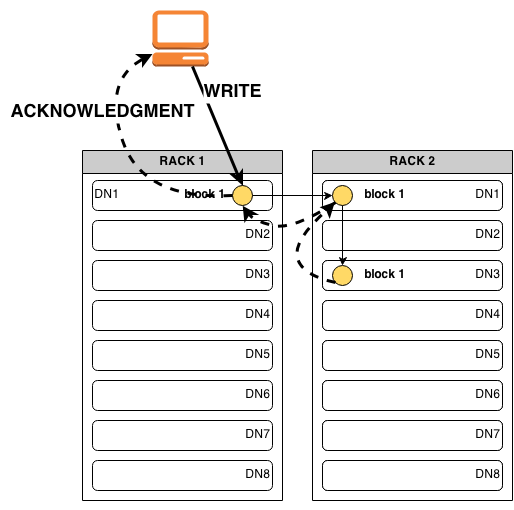
\includegraphics[width=4cm]{./Figures/chain_replication}}
    \column{5cm}
    \framebox{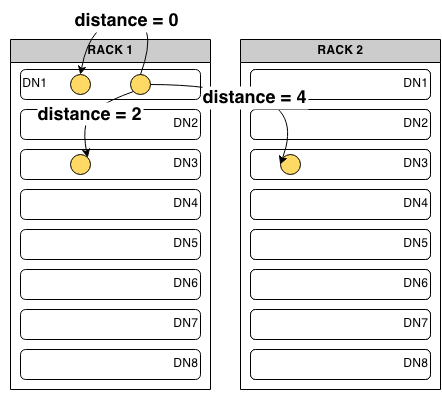
\includegraphics[width=4cm]{./Figures/hadoop_distance}}
  \end{columns}

}

%%%%%%%%%%%%%%%%%%%%%%%%%%%%%%%%%%%%%%%%%%%%%%%%%%%%%%%%%%
\frame {\frametitle{HDFS Coherency Model}
%%%%%%%%%%%%%%%%%%%%%%%%%%%%%%%%%%%%%%%%%%%%%%%%%%%%%%%%%%
  \begin{itemize}
  \item \textbf{Read your writes is not guaranteed}
    \begin{itemize}
    \item The namespace is updated
    \item Block contents may not be visible after a write is finished
    \item Application design (other than MapReduce) should use
      \texttt{sync()} to force synchronization
    \item \texttt{sync()} involves some overhead: tradeoff between
      robustness/consistency and throughput
    \end{itemize}

    \vspace{40pt}

  \item \textbf{Multiple writers (for the {\color{red}same} block) are not
    supported}
    \begin{itemize}
    \item Instead, different blocks can be written in parallel (using MapReduce)
    \end{itemize}

  \end{itemize}
}

